 \documentclass{beamer}
%
% Choose how your presentation looks.
% For more themes, color themes and font themes, see:
% http://deic.uab.es/~iblanes/beamer_gallery/index_by_theme.html
%
\mode<presentation>
{
  \usetheme{Madrid}      % or try Darmstadt, Madrid, Warsaw, ...
  \usecolortheme{seahorse} % or try albatross, beaver, crane, ...
  \usefonttheme{serif}  % or try serif, structurebold, ...
  \setbeamertemplate{navigation symbols}{}
  \setbeamertemplate{caption}[numbered]
  \usepackage{amsmath}
  \usepackage{tcolorbox}
  \usepackage[export]{adjustbox}
  \tcbuselibrary{most}
  \usepackage{arydshln}
  \usepackage{tikz}
  \usetikzlibrary{plotmarks}
  \usepackage{pgfplots}
  \newcommand{\Ivec}[1]{\mbox{\boldmath $#1$}}
    \usepackage[normalem]{ulem}
    % \usepackage{tipa}
    \newcommand{\git}{\texttt{\textbf{git}}\xspace}
    \usepackage{listings}
} 


\definecolor{myblue}{RGB}{65,105,225} 
\definecolor{myorange}{RGB}{250,190,0}

\setbeamercolor{structure}{fg=white,bg=myorange}
\setbeamercolor*{palette primary}{fg=myblue,bg=myorange}
\setbeamercolor*{palette secondary}{fg=white,bg=myblue}
\setbeamercolor*{palette tertiary}{bg=myblue,fg=white}
\setbeamercolor*{palette quaternary}{fg=white,bg=myorange!50}

\setbeamercolor{frametitle}{fg=black!90!myblue}

\setbeamercolor{section in head/foot}{fg=white,bg=myblue}
\setbeamercolor{author in head/foot}{fg=black,bg=myorange}
\setbeamercolor{title in head/foot}{fg=white,bg=myblue}

\setbeamertemplate{navigation symbols}{}

\setbeamertemplate{itemize/enumerate body begin}{\large}
\setbeamertemplate{itemize/enumerate subbody begin}{\large}


\defbeamertemplate*{headline}{mytheme}
{%
  \begin{beamercolorbox}[ht=2.25ex,dp=3.75ex]{section in head/foot}
    \insertnavigation{\paperwidth}
  \end{beamercolorbox}%
}%

\defbeamertemplate*{footline}{mytheme}
{
  \leavevmode%
  \hbox{%
  \begin{beamercolorbox}[wd=.5\paperwidth,ht=2.25ex,dp=1ex,right]{author in head/foot}%
    \usebeamerfont{author in head/foot}\insertshortauthor\hspace*{2em}
  \end{beamercolorbox}%
  \begin{beamercolorbox}[wd=.5\paperwidth,ht=2.25ex,dp=1ex,left]{title in head/foot}%
    \usebeamerfont{title in head/foot}\hspace*{2em}\insertshortsubtitle\hspace*{2em}
    \insertframenumber{} / \inserttotalframenumber
  \end{beamercolorbox}}%
  \vskip0pt%
}



\usepackage[english]{babel}
\usepackage[utf8x]{inputenc}
\usepackage{xcolor}
\usepackage{listings}
\usepackage{pgf}  
\usepackage{textpos}
\usepackage{tabulary}
\usepackage{scrextend}
\usepackage{hyperref}
\usepackage{setspace}
\usepackage{rotating}
\lstset
{
    language=[LaTeX]TeX,
    breaklines=true,
    basicstyle=\tt\scriptsize,
    %commentstyle=\color{green}
    keywordstyle=\color{blue},
    %stringstyle=\color{black}
    identifierstyle=\color{magenta},
}
\newcommand{\bftt}[1]{\textbf{\texttt{#1}}}
%\newcommand{\comment}[1]{{\color[HTML]{008080}\textit{\textbf{\texttt{#1}}}}}
\newcommand{\cmd}[1]{{\color[HTML]{008000}\bftt{#1}}}
\newcommand{\bs}{\char`\\}
\newcommand{\cmdbs}[1]{\cmd{\bs#1}}
\newcommand{\lcb}{\char '173}
\newcommand{\rcb}{\char '175}
\newcommand{\cmdbegin}[1]{\cmdbs{begin\lcb}\bftt{#1}\cmd{\rcb}}
\newcommand{\cmdend}[1]{\cmdbs{end\lcb}\bftt{#1}\cmd{\rcb}}

\newcommand{\wllogo}{\textbf{Overleaf}}

% this is where the example source files are loaded from
% do not include a trailing slash
\newcommand{\fileuri}{https://raw.githubusercontent.com/GiancarloSucci/A2023/main/A2022.IDSEPCLaTeX/}


\usepackage{stackengine}
\def\Ruble{\stackengine{.67ex}{%
  \stackengine{.48ex}{\textsf{P}}{\rule{.8ex}{.12ex}\kern.6ex}{O}{r}{F}{F}{L}%
  }{\rule{.8ex}{.12ex}\kern.6ex}{O}{r}{F}{F}{L}\kern-.1ex}



%----------------------------------------------------------------------------------------
%	TITLE PAGE
%----------------------------------------------------------------------------------------
\title[L02]{Introduzione alla data science e al pensiero computazionale\\
Lezione 2: La produzione del software nel lavoro (condiviso); gitHub} % The short title appears at the bottom of every slide, the full title is only on the title page

\author[{\tiny Giancarlo Succi }]{Giancarlo Succi\\\\ Dipartimento di Informatica -- Scienza e Ingegneria\\Universit\`{a} di Bologna\\
\bftt{g.succi@unibo.it}
} % Your name
\institute[unibo] % Your institution as it will appear on the bottom of every slide, may be shorthand to save space

\date{} % Date, can be changed to a custom date

\setbeamertemplate{navigation symbols}{}
\AtBeginSection[]
{
        \begin{frame}<beamer>{Outline}
                \tableofcontents[currentsection]
        \end{frame}
}

\begin{document}
\begin{frame}
\titlepage % Print the title page as the first slide

\end{frame}

%=============================================

\addtobeamertemplate{frametitle}{}{%
\begin{textblock*}{10mm}(-0.01mm,-0.95cm)

\includegraphics[width=0.9cm]{unibo-logo.png}
\end{textblock*}}

%=============================================

\begin{frame}
{\centerline{Piano della lezione}}
\begin{itemize}
    \item La produzione del software
    \item \git
\end{itemize} 
\end{frame}

\begin{frame}
{\centerline{Crediti per il materiale didattico}}
\begin{itemize}
    \item Il materiale didattico relativo a \textcolor{red}{\git} \`{e} basato sull'introduzione a \git ~ del \textcolor{blue}{dott. Emanuele Olivetti}, che ha gentilmente concesso il suo uso
    \item La localizzazione dell'originale \`{e} \url{https://github.com/emanuele/introduction_to_Git}
\end{itemize} 
\end{frame}


\begin{frame}
{\centerline{La produzione del software}}
\begin{itemize}
    \item Il software \`{e} un bene immateriale
    \item \`{E} un po' come la musica
    \item Produrlo insieme ad altre persone apparirebbe essere pi\`{u} semplice
    \begin{itemize}
    \item in modo ingenuo si potrebbe pensare che basterebbe scambiarsi il codice
    \item per questo in ogni caso il lavoro remoto e lo sviluppo distribuito su scala planetaria sono pratiche non solo comune, ma, alle volte, molto profittevoli
    \item vi sono persino ditte virtuali di grande successo
\end{itemize} 
\item Allo stesso modo i musicisti potrebbero scambiarsi gli spartiti online
\end{itemize} 
\end{frame}

\begin{frame}
{\centerline{Il problema nella produzione del software (1/2)}}
\begin{itemize}
    \item Avete mai provato a scambiarvi una traduzione di latino online o per telefono?
    \item Che cosa succede spesso?
    \begin{itemize}
    \item Non ci si ricorda qual \`{e} la copia giusta
    \item Se ci sono errori, spesso non si capisce chi lo ha commesso
    \item Ci sono difficolt\`{a} a dare credito a chi ha fatto la mole principale di lavoro
\end{itemize} 

\end{itemize} 
\end{frame}

\begin{frame}
{\centerline{Il problema nella produzione del software (2/2)}}
\begin{itemize}
    \item Tutto questo, e ancora molto di pi\`{u} succede nel software
    \item E per noi per ora il testo dei lucidi \`{e} il software
    \item E vedete come \`{e} difficile recuperare la versione pi\`{u} recente e corretta, e qual \`{e} il rischio di sbagliare date, aula, indirizzi email, ecc
\end{itemize} 
\end{frame}

\begin{frame}
{\centerline{\git}}
\begin{itemize}
    \item Per questo si usano sistemi di sincronizzazione del lavoro condiviso, detti ``sistemi di gestione delle versioni''
    \item Essi \textcolor{red}{\textbf{NON}} risolvono il problema di come sviluppare il software da soli o con altri
    \item Per\`{o} danno un contributo \textcolor{orange}{\textbf{ESSENZIALE}} al lavoro
    \item Per questo il loro uso sar\`{a} un aspetto centrale del corso
\end{itemize} 
\end{frame}

\begin{frame}{\centerline{Outline}}
  \begin{itemize}
  \item Version Control: \git.
  \item Scenario 1: \textbf{singolo} sviluppatore, 
    repository \textbf{locale}.
  \item Scenario 2: \textbf{Team} di sviluppatori, repository \textbf{centralizzato e remoto}. Minimalistico.
  \item Branching.
  \item Scenario 3: Contribuire a un progetto software localizzato su
    \textbf{GitHub}.
  \item Extra: come organizzare un repository centralizzato e pi\`{u}.
  \end{itemize}
\end{frame}

\begin{frame}{\centerline{Version Control: Nomi \& Significato}}
  \begin{block}{Da Wikipedia in inglese}
    ``\emph{Il sistema di gestione delle revisioni}, anche conosciuto come \emph{version control},
    \emph{source control} o, in parte, \emph{software configuration management}
    (SCM), \`{e} \alert{la modalit\`{a} di gestione dei cambi a documenti, programmi e altre informazioni salvate come file su computer}.''
  \end{block}
  Acronimi in uso:
  \begin{itemize}
  \item VC
  \item SCM
  \end{itemize}
  Errori di denominazione:
  \begin{itemize}
  \item \sout{Versioning}
  \end{itemize}
  \textbf{D:} Avete mai usato un sistema di VC?
\end{frame}

\begin{frame}{\centerline{VC: Locale, Centralizzato, Distribuito}}
\begin{center}
  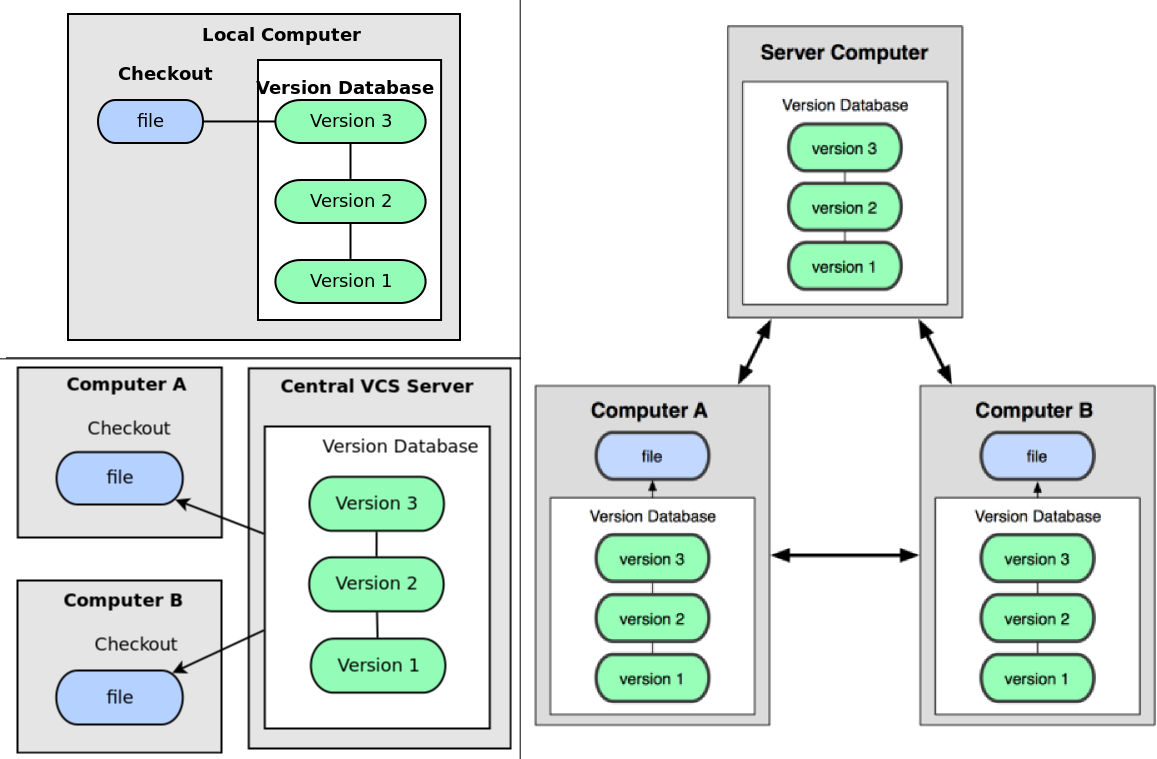
\includegraphics[width=0.8\linewidth]{A2023.LavoroCondiviso/vc_paradigms}
\\
\small
Da \emph{Pro Git}, S.Chacon 2009, CC 3.0 license.
\end{center}
\end{frame}



\begin{frame}{\centerline{Sondaggio: \git}}
  \begin{itemize}\setlength{\itemsep}{+3mm}
  \item D1: Avete mai sentito parlare di \git?
  \item D2: Usate \git?
  \item D3: Da dove viene il nome ``\git''? (dalla FAQ di \git)
    \begin{enumerate}\setlength{\itemsep}{+2mm}
    \item Una combinazione di tre lettere a caso che \`{e} pronunciabile.
    \item Acronimo (global information tracker).
    \item Ironia.
    \end{enumerate}
  \end{itemize}
\end{frame}

\begin{frame}{\centerline{\git? Perch\'{e} ``\git''?}}
  \begin{columns}
    \begin{column}{5cm}
      \textbf{Linus Torvalds}: 
        \emph{``Io assegno nomi a tutti i miei progetti da me, prima Linux e ora
        \git.}''
      \begin{figure}
        \centering
        \includegraphics[width=4cm]{A2023.LavoroCondiviso/Linus_Torval';.ds}
      \end{figure}
    \end{column}
    \begin{column}{7cm}
      \begin{figure}
        \url{http://www.merriam-webster.com/dictionary/git}
        \centering
        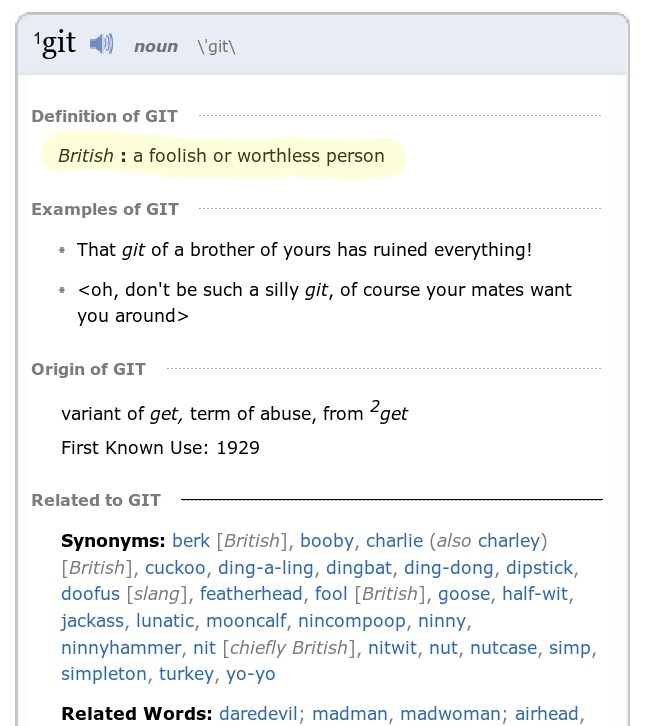
\includegraphics[width=5cm]{A2023.LavoroCondiviso/git-merriam}
      \end{figure}
    \end{column}
    \end{columns}
\end{frame}


\begin{frame}[containsverbatim]{\centerline{\git (1/2)}}
  \begin{center}
  Dalla pagina del manuale (in inglese):
  \item \texttt{\textbf{git}}
  \end{center}
\begin{verbatim}
usage: git [OPTIONS] COMMAND [ARGS]

The most commonly used git commands are:
   add        Add file contents to the index
   commit     Record changes to the repository
   diff       Show changes between commits, commit and working tree, etc
   ...
\end{verbatim}
  \begin{center}
    \texttt{\textbf{git help <command>}}
  \end{center}
  \begin{center}
    \texttt{\textbf{git status}}
  \end{center}
\end{frame}

\begin{frame}{\centerline{\git (2/2)}}
  Presentatevi a \git:
  \begin{center}
    \small
    \texttt{\textbf{git config -{}-global user.name "Emanuele Olivetti"}}
  \end{center}
  \vspace{0.2cm}
  \begin{center}
    \small
    \texttt{\textbf{git config -{}-global user.email "olivetti@fbk.eu"}}
  \end{center}
\end{frame}

\begin{frame}{\centerline{\git -- Singolo sviluppatore + repository locale}}
  \begin{figure}
    \centering
    Scenario 1: singolo sviluppatore + repository locale
  \end{figure}
\end{frame}

\begin{frame}{\centerline{ \git ~ -- Singolo+Locale -- Motivazioni}}
  \begin{itemize}\setlength{\itemsep}{+3mm}
  \item Per caso usate un VC per il vostro repository locale?
  \item Perch\'{e} usare un VC per un singolo sviluppatore con un repository locale?
    \begin{itemize}\setlength{\itemsep}{+2mm}
    \item Primo passo per un progetto condiviso.
    \item Backup.
    \item Per tracciare il proprio lavoro.
    \end{itemize}
  \end{itemize}
\end{frame}

\begin{frame}{\centerline{ \git ~ -- Singolo+Locale -- Init}}
  \begin{center}
    \texttt{\textbf{git init}}
  \end{center}
  \begin{itemize}
  \item Crea un repository \git ~ vuoto.
  \item Crea una directory \git: ~ \texttt{.git/}
  \end{itemize}
  \begin{figure}
    \centering
    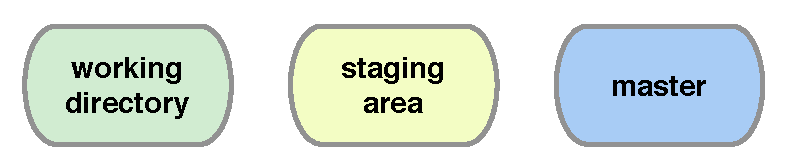
\includegraphics[width=9cm]{A2023.LavoroCondiviso/local-init}
  \end{figure}
  Nota: \`{e} una azione \textcolor{red}{sicura}. Non cambia i file esistenti.
\end{frame}

\begin{frame}{\centerline{ \git ~ -- Singolo+Locale -- Il flusso dei dati}}
  \begin{center}
    \texttt{\textbf{git add <filename>}}
  \end{center}
  \begin{figure}
    \centering
    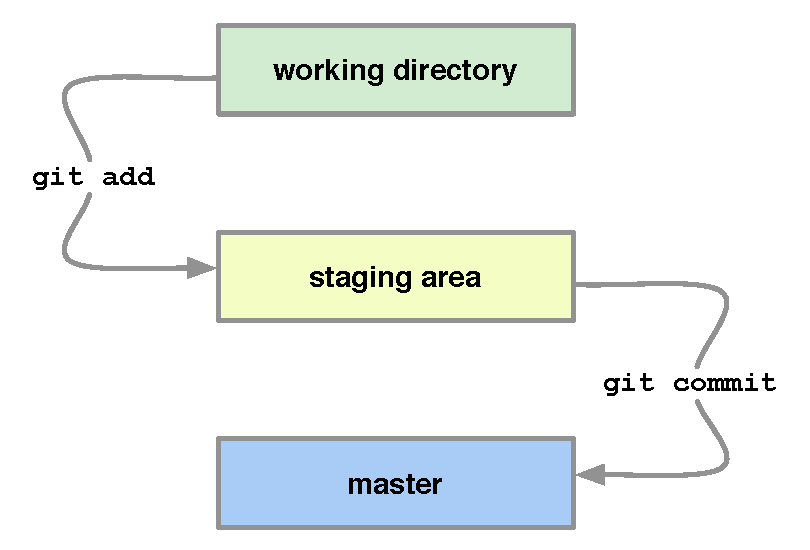
\includegraphics[width=5.5cm]{A2023.LavoroCondiviso/staging}
  \end{figure}
  \begin{center}
    \texttt{\textbf{git commit -m "Let us begin."}}
  \end{center}

  \begin{block}{Wikipedia (tradotto dall'inglese)}
    ``La \emph{staging area} \`{e} il luogo dove organismi, persone, veicoli, equipaggiamenti o materiali sono messi insieme prima dell'uso''.
  \end{block}
\end{frame}

\begin{frame}{\centerline{ \git ~ -- Singolo+Locale -- Add}}
  \begin{center}
    \texttt{\textbf{git add file1 [file2 ...]}}
  \end{center}
  \begin{itemize}
  \item Aggiunge nuovi file per il successivo \texttt{commit}.
  \item Aggiunge contenuto dalla directory di lavoro alla staging area per il successivo commit, in pratica indicizza
  \item Non aggiunge informazioni sui permessi dei file
  \item Di per s\'{e} non crea directory
  \end{itemize}
  \begin{figure}
    \centering
    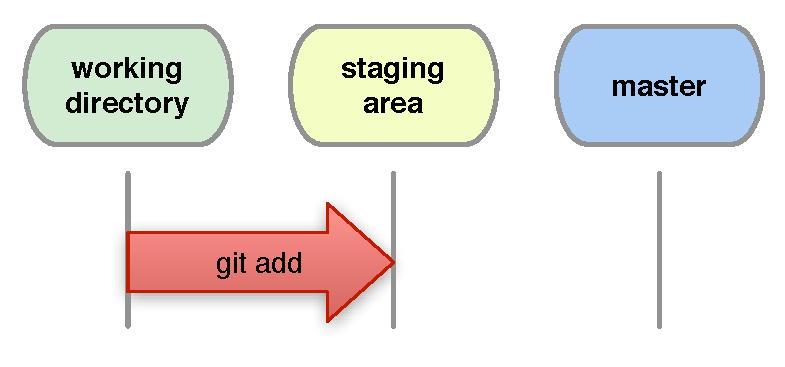
\includegraphics[width=7cm]{A2023.LavoroCondiviso/local-add}
  \end{figure}
\end{frame}

\begin{frame}{\centerline{ \git ~ -- Singolo+Locale -- Commit (1/2)}}
  \begin{center}
    \texttt{\textbf{git commit [-m "Commit message."]}}
  \end{center}
  Trascrive tutti i cambiamenti dalla staging area al master.
  \begin{figure}
    \centering
    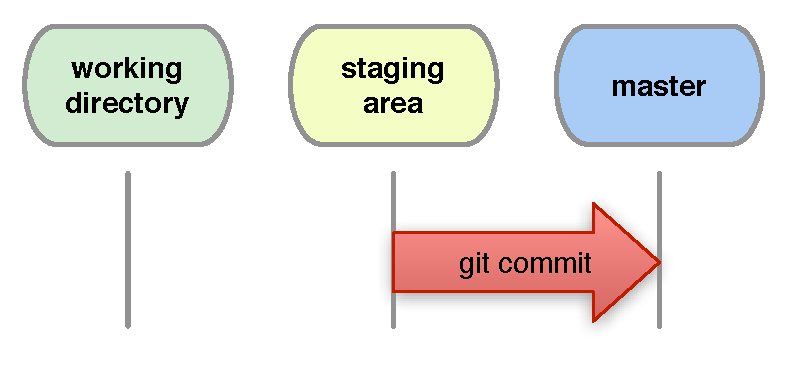
\includegraphics[width=9cm]{A2023.LavoroCondiviso/local-commit}
  \end{figure}
\end{frame}

\begin{frame}{\centerline{ \git ~ -- Singolo+Locale -- Commit (2/2)}}
  \begin{center}
    \texttt{\textbf{git commit file1 file2}}
  \end{center}
  Trascrive i cambiamenti dalla directory di lavoro e dalla staging area al master per \texttt{\textbf{file1}},
  \texttt{\textbf{file2}} 
  \begin{figure}
    \centering
    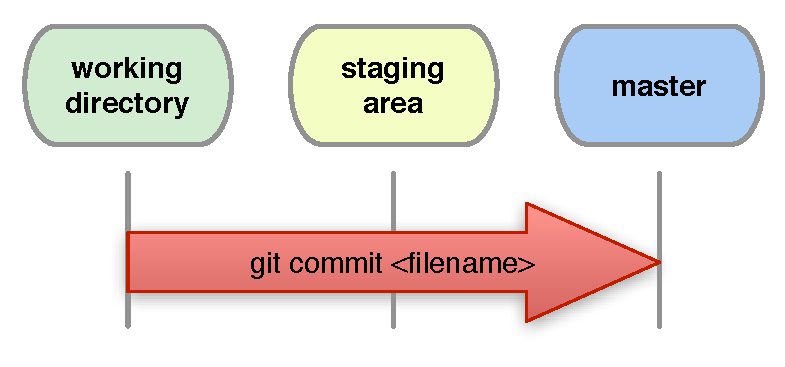
\includegraphics[width=9cm]{A2023.LavoroCondiviso/local-commit-filename}
  \end{figure}
  \begin{center}
    \texttt{\textbf{git commit -a}}
  \end{center}
  \textcolor{red}{Attenzione! } Trascrive tutti i cambiamenti nella directory di lavoro e nella staging area
\end{frame}

\begin{frame}{\centerline{ \git ~ -- Singolo+Locale -- Diff }}
  \begin{center}
    \texttt{\textbf{git diff}}
  \end{center}
  Presenta quali cambiamenti siano present tra la \emph{directory di lavoro} e la
  \emph{staging area}; lavora sugli indici
  \begin{figure}
    \centering
    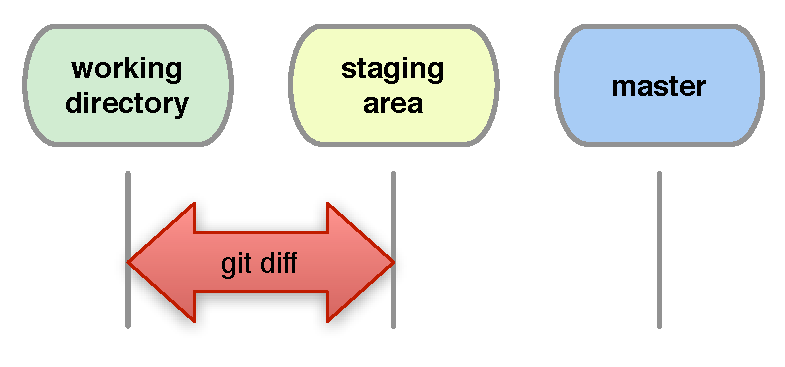
\includegraphics[width=9cm]{A2023.LavoroCondiviso/local-diff}
  \end{figure}
\end{frame}

\begin{frame}{\centerline{ \git ~ -- Singolo+Locale -- Logs (1/2)}}
  \begin{center}
    \texttt{\textbf{git log}}
  \end{center}
  Presenta i dettagli dei commit; ecco perch\'{e} servono i messaggi
  \begin{figure}
    \centering
    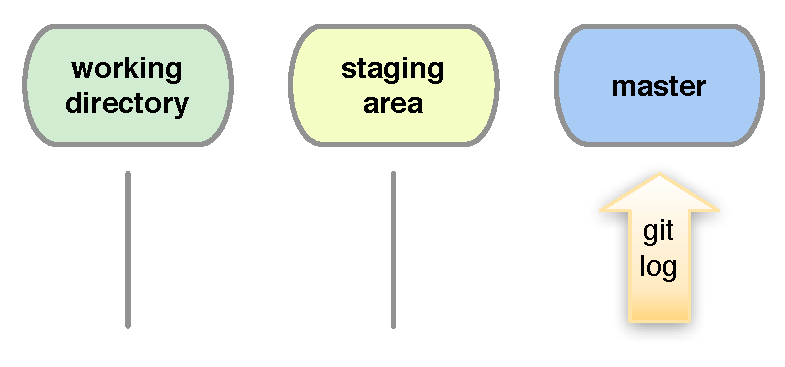
\includegraphics[width=9cm]{A2023.LavoroCondiviso/local-log}
  \end{figure}
\end{frame}

\begin{frame}{\centerline{ \git ~ -- Singolo+Locale -- Logs (2/2) }}
  \begin{center}
    \texttt{\textbf{gitk}}
  \end{center}
  Interfaccia grafica per navigare in un repository \git:
  \begin{figure}
    \centering
    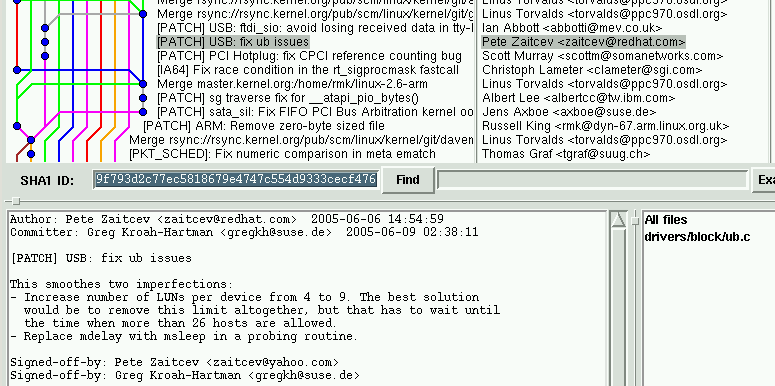
\includegraphics[width=9.4cm]{A2023.LavoroCondiviso/gitk_cropped}
  \end{figure}
\end{frame}


\begin{frame}{\centerline{\git ~ -- Team+Remoto/Condiviso (1/3)}}
  \begin{figure}
    \centering
    Scenario 2: \textbf{Team} di sviluppatori, repository \textbf{centralizzato e remoto}. Minimalistico.
  \end{figure}
\end{frame}

\begin{frame}{\centerline{\git ~ -- Team+Remoto/Condiviso (2/3)}}
  \begin{figure}
    \centering
    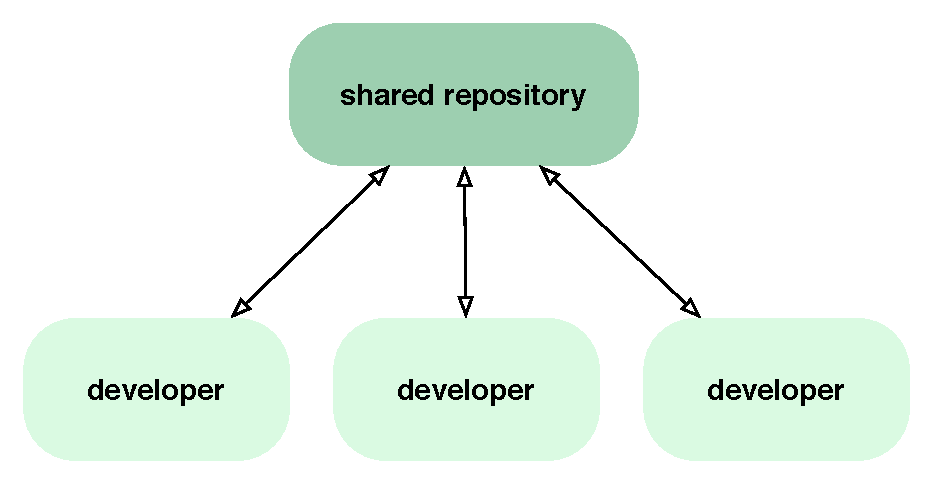
\includegraphics[width=10cm]{A2023.LavoroCondiviso/workflow-a}
  \end{figure}
\end{frame}

\begin{frame}{\centerline{\git ~ -- Team+Remoto/Condiviso (3/3)}}
  \begin{figure}
    \centering
    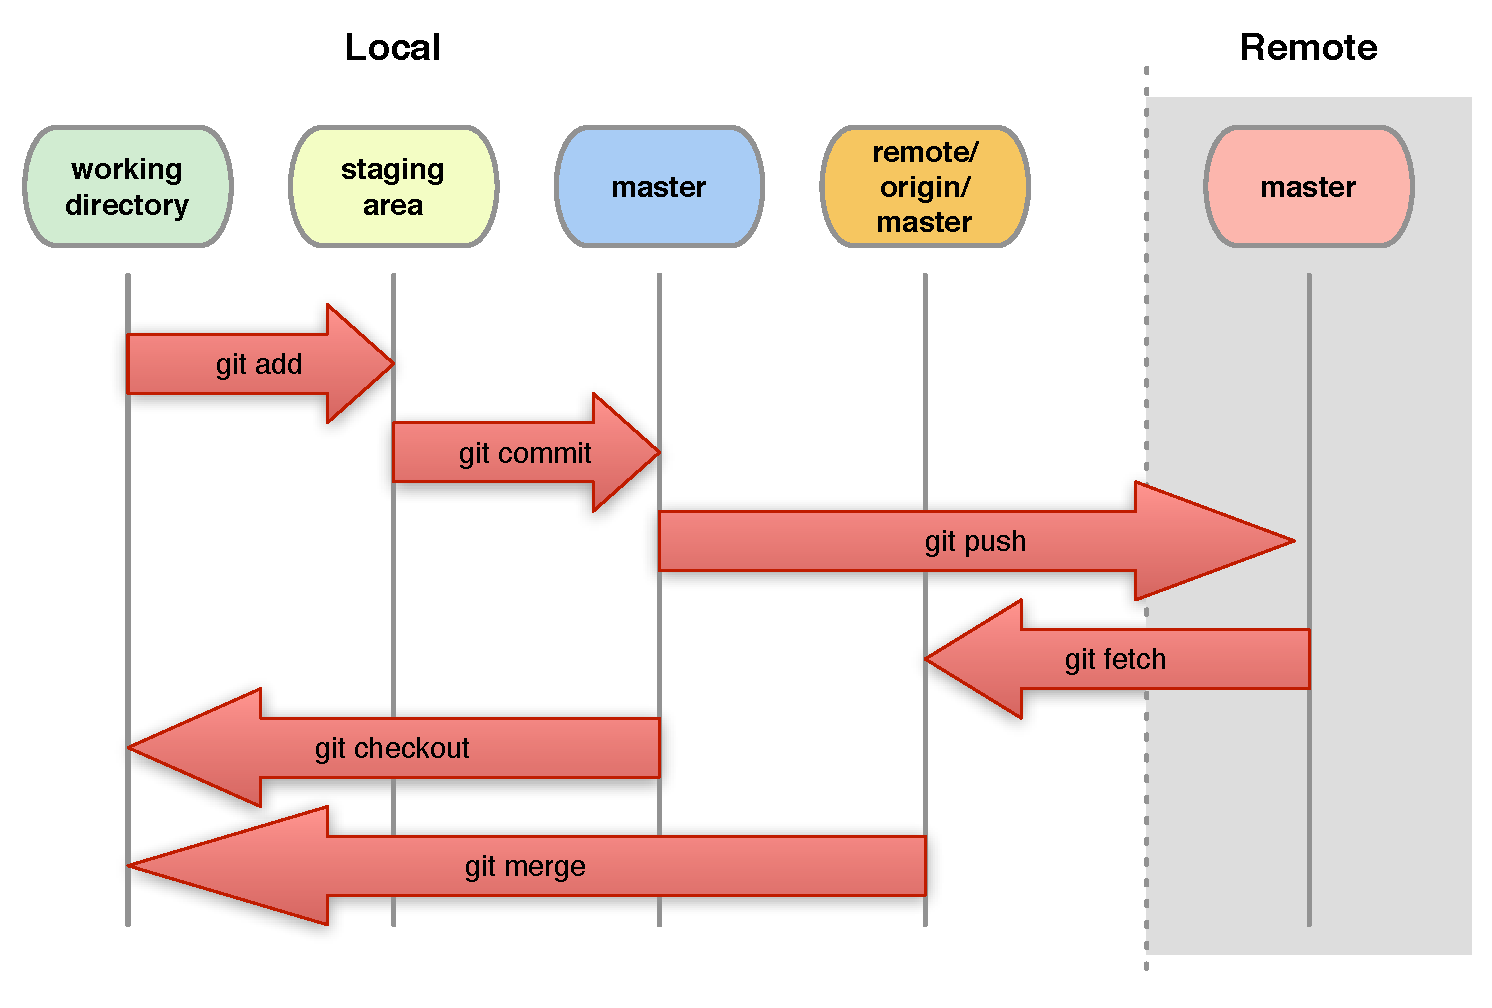
\includegraphics[width=11cm]{A2023.LavoroCondiviso/local-remote}
  \end{figure}  
\end{frame}

\begin{frame}{\centerline{\git ~ -- Team+Remoto/Condiviso  -- Passi}}
  \begin{center}
    \texttt{\textbf{git clone <URL>}}
  \end{center}
  \uncover<2->{Crea \alert{\emph{due}} copie locali di
    \alert{tutto} il repository remoto.}
  \begin{figure}
    \begin{center}
      \includegraphics<1>[width=9cm]{A2023.LavoroCondiviso/local-remote-before-clone}
      \includegraphics<2>[width=9cm]{A2023.LavoroCondiviso/local-remote-clone2}
    \end{center}
  \end{figure}
  \uncover<2->{Protocolli di trasmissione dati disponibili:
  \begin{itemize}
  \item \texttt{\textbf{ssh://}}, \texttt{\textbf{git://}},
    \texttt{\textbf{http://}}, \texttt{\textbf{https://}},
    \texttt{\textbf{file://}}
  \end{itemize}
  Es.: \small{\texttt{\textbf{git clone https://github.com/ASPP/pelita.git}}}
  \begin{center}
    \texttt{\textbf{git remote -v}}
  \end{center}
  mostra \textbf{nome} e \texttt{\textbf{URL}} del repository remoto.}
\end{frame}

\begin{frame}{\centerline{\git ~ -- Team+Remoto/Condiviso  -- Fetch}}
  \begin{center}
    \texttt{\textbf{git fetch}}
  \end{center}
  \begin{itemize}
  \item Scarica gli aggiornamenti dal master remoto al master locale.
  \item Il master locale, la staging area e la directory di lavoro non cambiano.
  \end{itemize}
  \begin{figure}
    \centering
    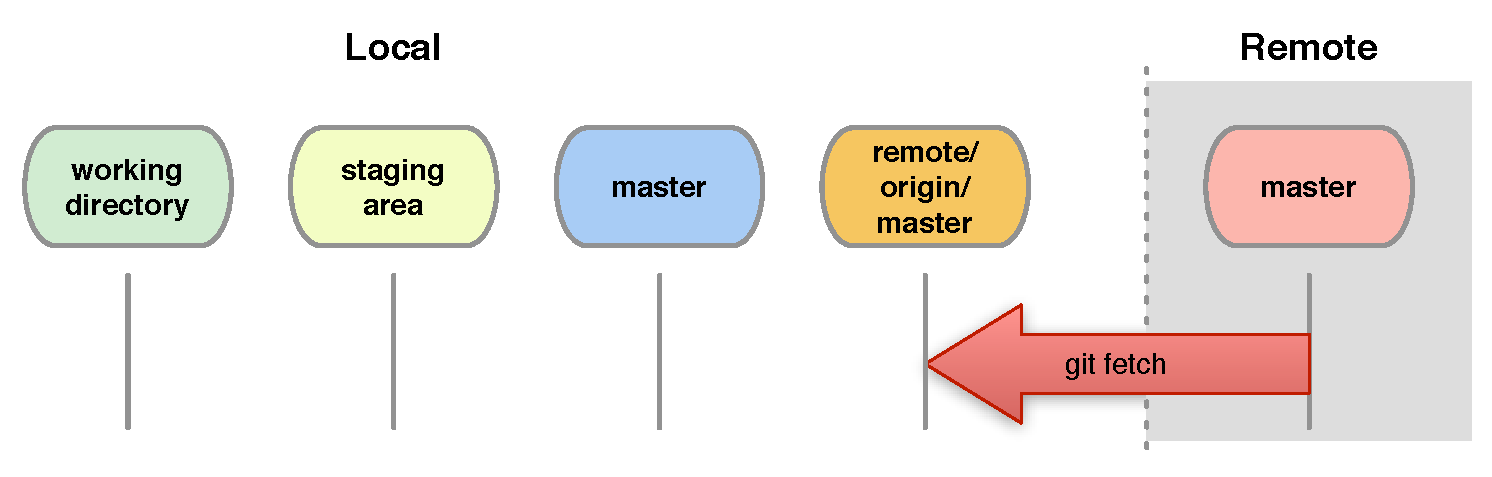
\includegraphics[width=9.5cm]{A2023.LavoroCondiviso/local-remote-fetch}
  \end{figure}
\end{frame}


\begin{frame}{\centerline{\git ~ -- Team+Remoto/Condiviso  -- Merge}}
  \begin{center}
    \texttt{\textbf{git merge}}
  \end{center}
  \begin{itemize}
  \item Permette di riunire flussi di sviluppo diversi.
  \item \alert{Attenzione}: pu\`{o} generare \emph{conflitti}!
  \item \textcolor{orange}{Nota}: La riunione (merge) avviene solo quando i cambiamenti sono stati sottoposti a commit.
  \end{itemize}
  \begin{figure}
    \centering
    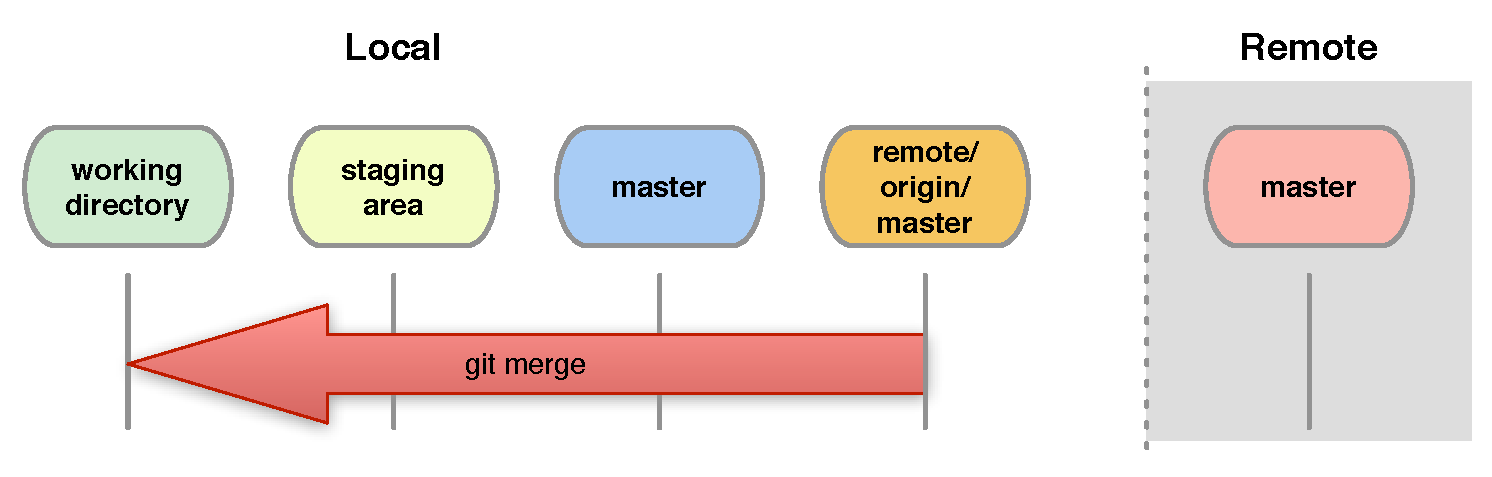
\includegraphics[width=9.5cm]{A2023.LavoroCondiviso/local-remote-merge}
  \end{figure}
  \begin{center}
    \texttt{\textbf{git fetch}} + \texttt{\textbf{git merge}} = \texttt{\textbf{git pull}}
  \end{center}
\end{frame}

\begin{frame}[containsverbatim]{\centerline{\git ~ -- Team+Remoto/Condiviso  -- Conflitti (1/2)}}
  \begin{center}
    \alert{Conflitti!}
  \end{center}
\begin{verbatim}
  ...
  <<<<<<< yours:sample.txt
  Conflict resolution is hard;
  let's go shopping.
  =======
  Git makes conflict resolution easy.
  >>>>>>> theirs:sample.txt
  ...
\end{verbatim}
\end{frame}


\begin{frame}{\centerline{\git ~ -- Team+Remoto/Condiviso  -- Conflitti (2/2)}}
Risoluzione dei conflitti
\begin{enumerate}
\item Bisogna innanzitutto vedere dove sono i conflitti:
  \begin{center}
  \texttt{\textbf{git diff}}
  \end{center}
\item Poi occorre modificare le linee che provocano conflitto.
\item Quindi si aggiungono le modifiche alla staging area:
  \begin{center}
    \texttt{\textbf{git add file1 [...]}}
  \end{center}
\item E quindi si ripete un commit:
  \begin{center}
    \texttt{\textbf{git commit -m "Conflicts solved."}}
  \end{center}
\end{enumerate}
\end{frame}

\begin{frame}{\centerline{\git ~ -- Team+Remoto/Condiviso  -- Push}}
  \begin{center}
    \texttt{\textbf{git push}}
  \end{center}
  \begin{itemize}
  \item Modifica i \emph{remote masters} (sia locale che remoto).
  \item Occorre prima di tutto fare un \texttt{\textbf{fetch}}+\texttt{\textbf{merge}}
  \item Solo dopo si pu\`{o} fare un push.
  \end{itemize}
  \begin{figure}
    \centering
    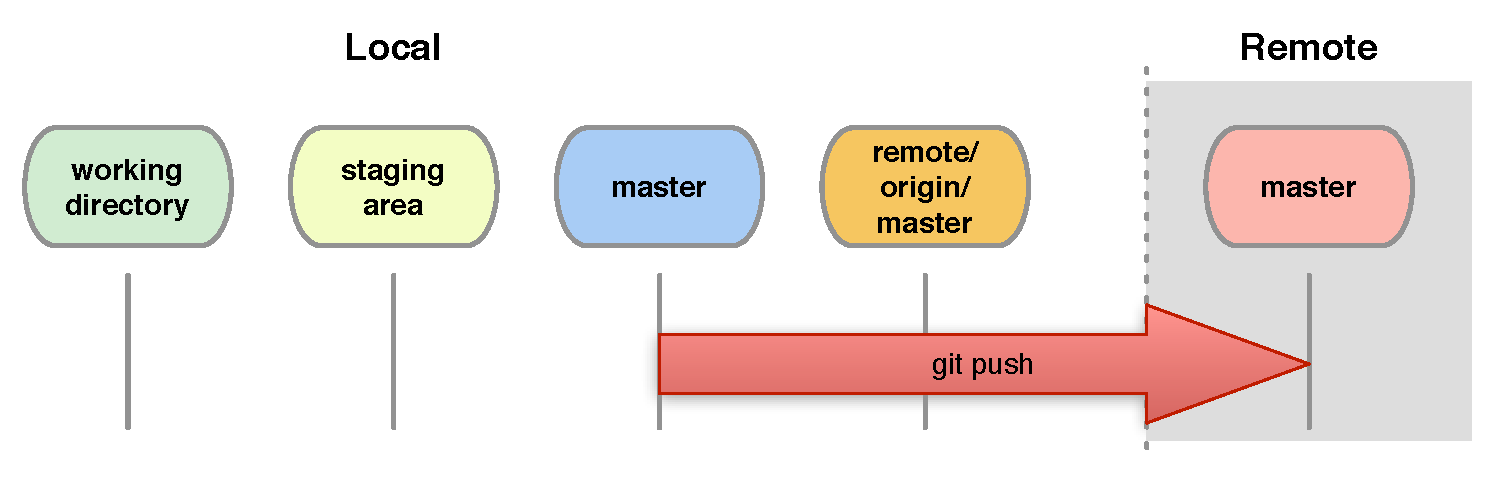
\includegraphics[width=9.5cm]{A2023.LavoroCondiviso/local-remote-push}
  \end{figure}
\end{frame}

\begin{frame}{\centerline{Branching}}
  \begin{figure}
    \centering
    I fondamenti del branching, ovvero la suddivisione del prodotto per gestire configurazioni diverse
  \end{figure}
\end{frame}

\begin{frame}{\centerline{Dinamica del branching -- partenza}}
  \begin{columns}
    \begin{column}{0.6\linewidth}
      \begin{center}
        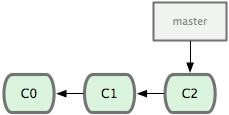
\includegraphics[width=6cm]{A2023.LavoroCondiviso/18333fig0310-tn}
      \end{center}
    \end{column}
    \begin{column}{0.4\linewidth}
      \begin{center}
        \texttt{\textbf{git commit (C0)}}\\
        \texttt{\textbf{git commit (C1)}}\\
        \texttt{\textbf{git commit (C2)}}
      \end{center}
    \end{column}
  \end{columns}
  \vspace{1em}
  \begin{center}
    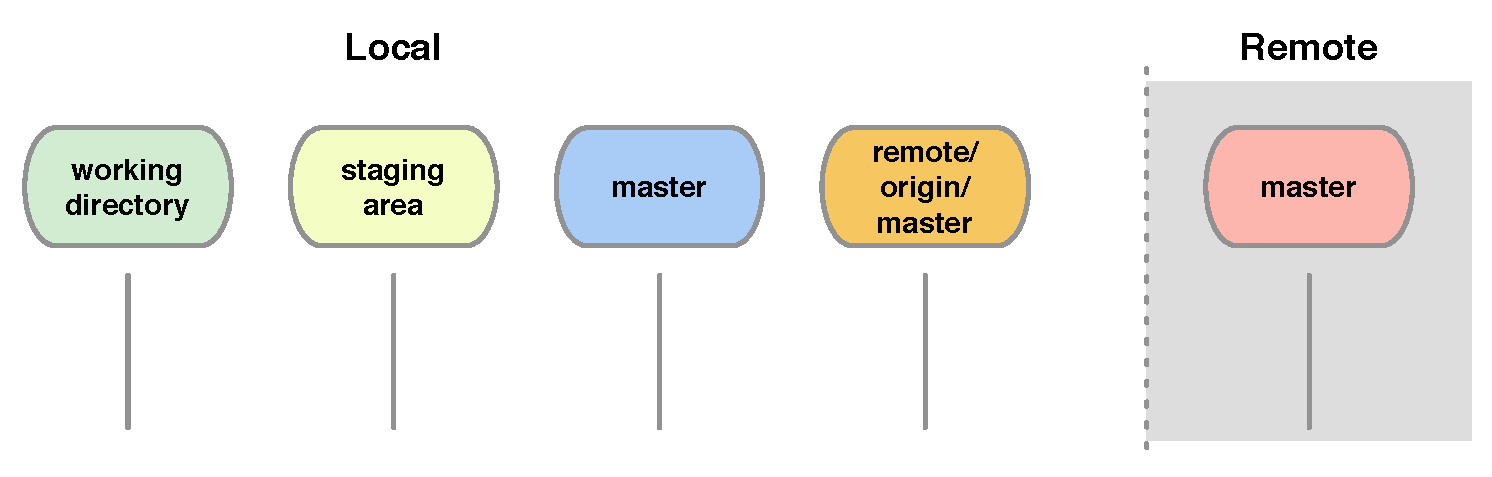
\includegraphics[width=9cm]{A2023.LavoroCondiviso/local-remote-clone}
  \end{center}
\end{frame}

\begin{frame}{\centerline{Dinamica del branching -- evoluzione (1/3)}}
  \begin{columns}
    \begin{column}{0.6\linewidth}
      \begin{center}
        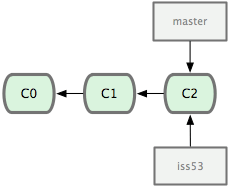
\includegraphics[width=4cm]{A2023.LavoroCondiviso/18333fig0311-tn}
      \end{center}
    \end{column}
    \begin{column}{0.45\linewidth}
        \texttt{\textbf{git branch iss53}}\\
    \end{column}
  \end{columns}
  \begin{center}
    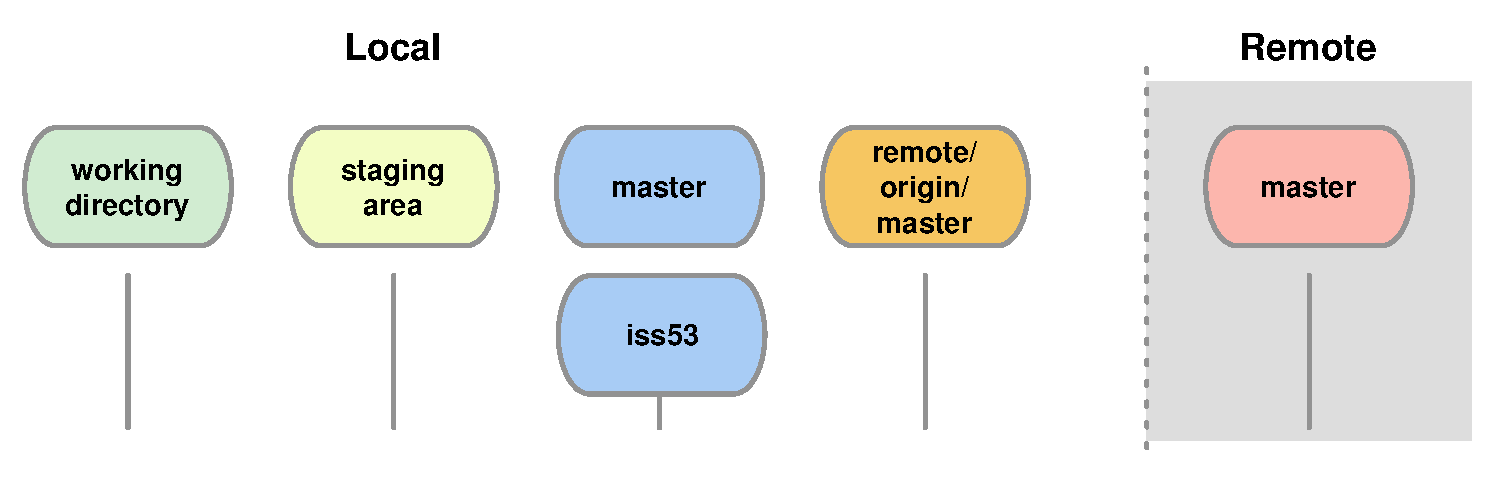
\includegraphics[width=8cm]{A2023.LavoroCondiviso/git-branch}
  \end{center}
\end{frame}

\begin{frame}{\centerline{Dinamica del branching -- evoluzione (2/3)}}
  \begin{columns}
    \begin{column}{0.6\linewidth}
      \begin{center}
        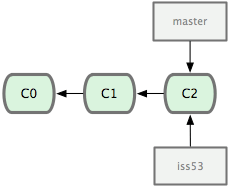
\includegraphics[width=4cm]{A2023.LavoroCondiviso/18333fig0311-tn}
      \end{center}
    \end{column}
    \begin{column}{0.45\linewidth}
        \texttt{\textbf{git branch iss53}}\\
        \texttt{\textbf{git checkout iss53}}\\
    \end{column}
  \end{columns}
  \begin{center}
    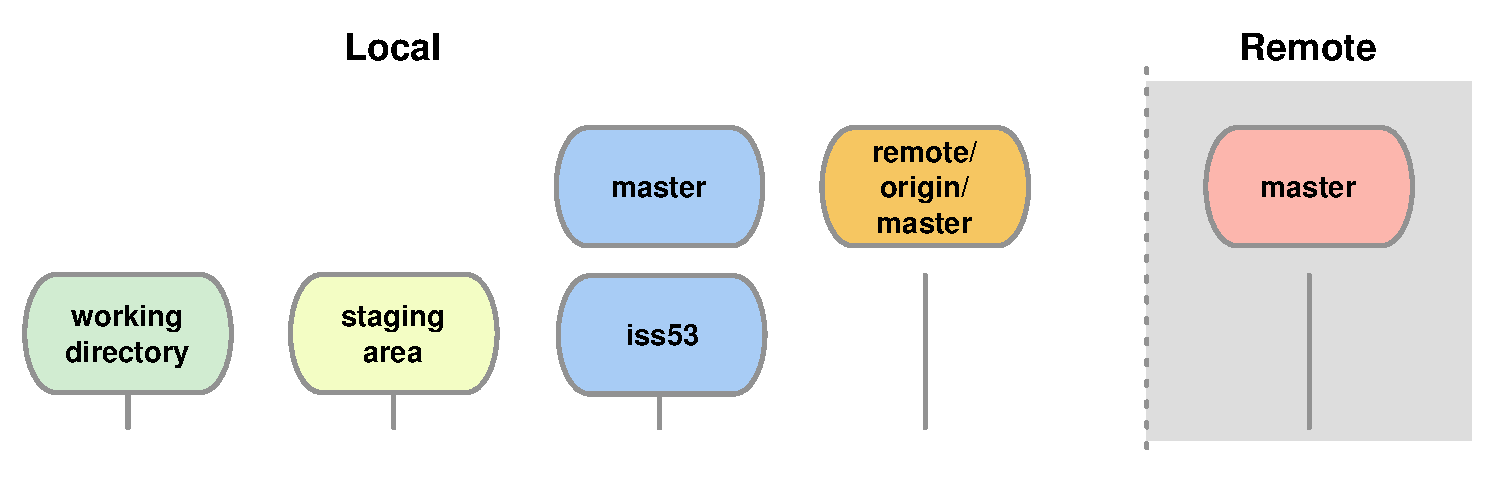
\includegraphics[width=8cm]{A2023.LavoroCondiviso/git-checkout}
  \end{center}
\end{frame}


\begin{frame}{\centerline{Dinamica del branching -- evoluzione (3/3)}}
  \begin{columns}
    \begin{column}{0.6\linewidth}
      \begin{center}
        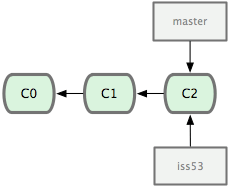
\includegraphics[width=4cm]{A2023.LavoroCondiviso/18333fig0311-tn}
      \end{center}
    \end{column}
    \begin{column}{0.45\linewidth}
        \texttt{\textbf{git branch iss53}}\\
        \texttt{\textbf{git checkout iss53}}\\
        \texttt{\textbf{git checkout master}}
    \end{column}
  \end{columns}
  \begin{center}
    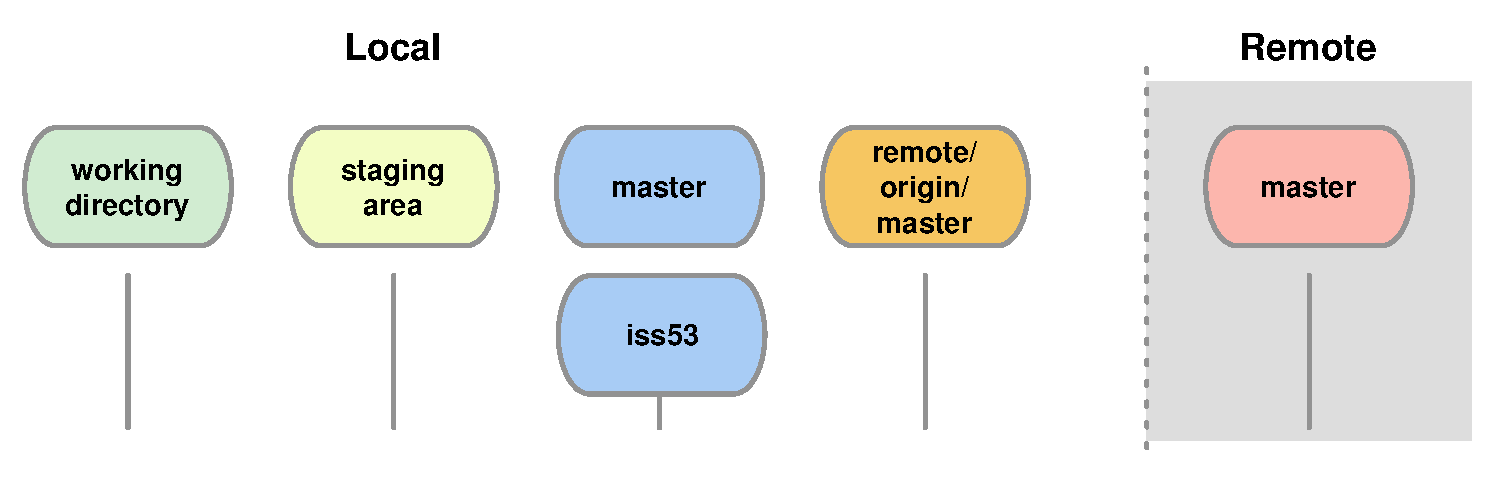
\includegraphics[width=8cm]{A2023.LavoroCondiviso/git-branch}
  \end{center}
\end{frame}

\begin{frame}{\centerline{Dinamica del branching -- nuovo commit}}
  \begin{columns}
    \begin{column}{0.6\linewidth}
      \begin{center}
        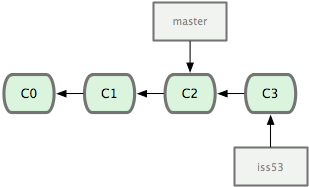
\includegraphics[width=6cm]{A2023.LavoroCondiviso/18333fig0312-tn}
      \end{center}
    \end{column}
    \begin{column}{0.4\linewidth}
      \begin{center}
        \texttt{\textbf{git checkout iss53}}\\
        \texttt{\textbf{git commit (C3)}}
      \end{center}
    \end{column}
  \end{columns}
  \begin{center}
    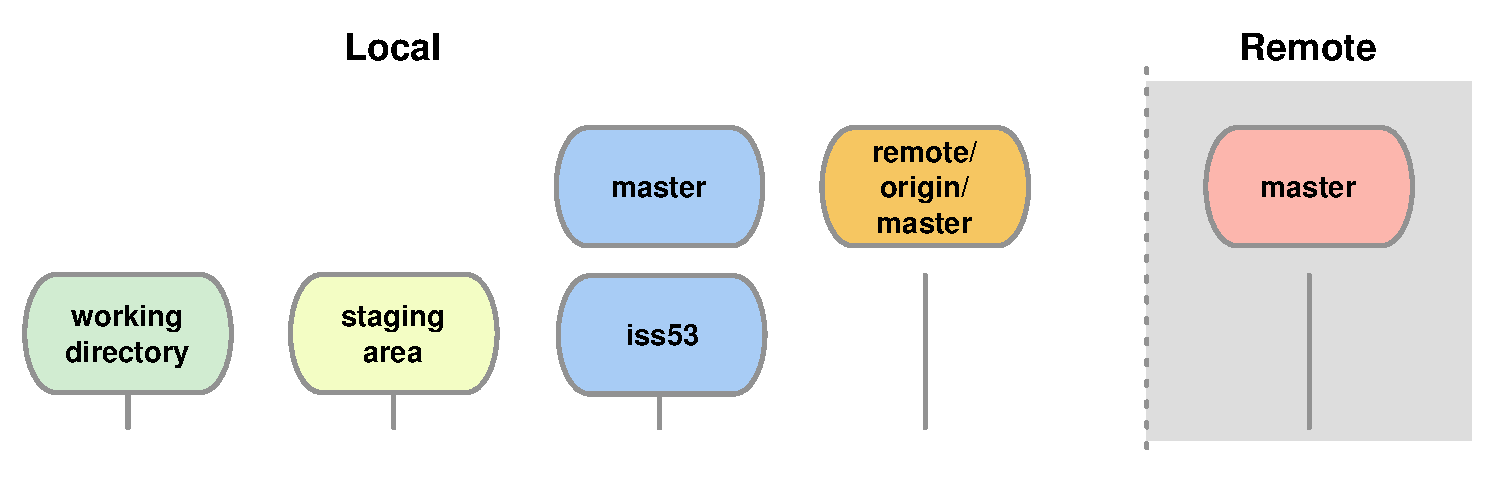
\includegraphics[width=7cm]{A2023.LavoroCondiviso/git-checkout}
  \end{center}
\end{frame}

\begin{frame}{\centerline{Dinamica del branching -- fix (1/2)}}
  \begin{columns}
    \begin{column}{0.6\linewidth}
      \begin{center}
        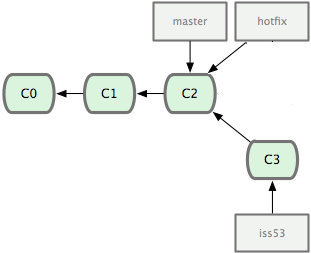
\includegraphics[width=4.5cm]{A2023.LavoroCondiviso/18333fig0313b-tn}
      \end{center}
    \end{column}
    \begin{column}{0.45\linewidth}
      \begin{center}
        \texttt{\textbf{git branch hotfix}}\\
      \end{center}
    \end{column}
  \end{columns}
  \begin{center}
    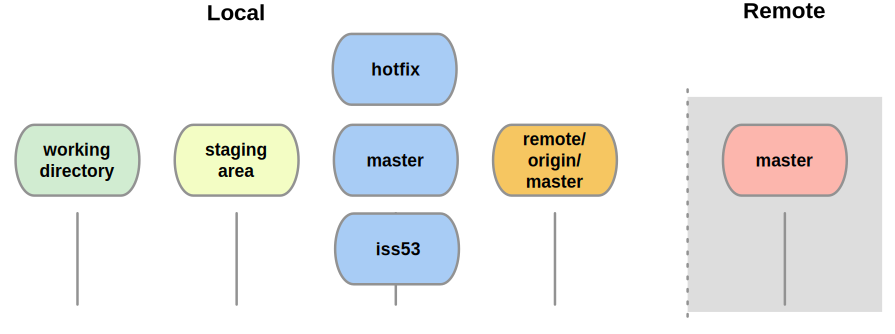
\includegraphics[width=6.5cm]{A2023.LavoroCondiviso/git-branch2}
  \end{center}
\end{frame}

\begin{frame}{\centerline{Dinamica del branching -- fix (2/2)}}
  \begin{columns}
    \begin{column}{0.6\linewidth}
      \begin{center}
        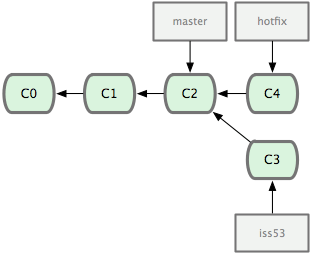
\includegraphics[width=5cm]{A2023.LavoroCondiviso/18333fig0313-tn}
      \end{center}
    \end{column}
    \begin{column}{0.45\linewidth}
      \begin{center}
        \uncover\texttt{\textbf{git checkout hotfix}}\\
        \uncover\texttt{\textbf{git commit (C4)}}\\
      \end{center}
    \end{column}
  \end{columns}
  \begin{center}
    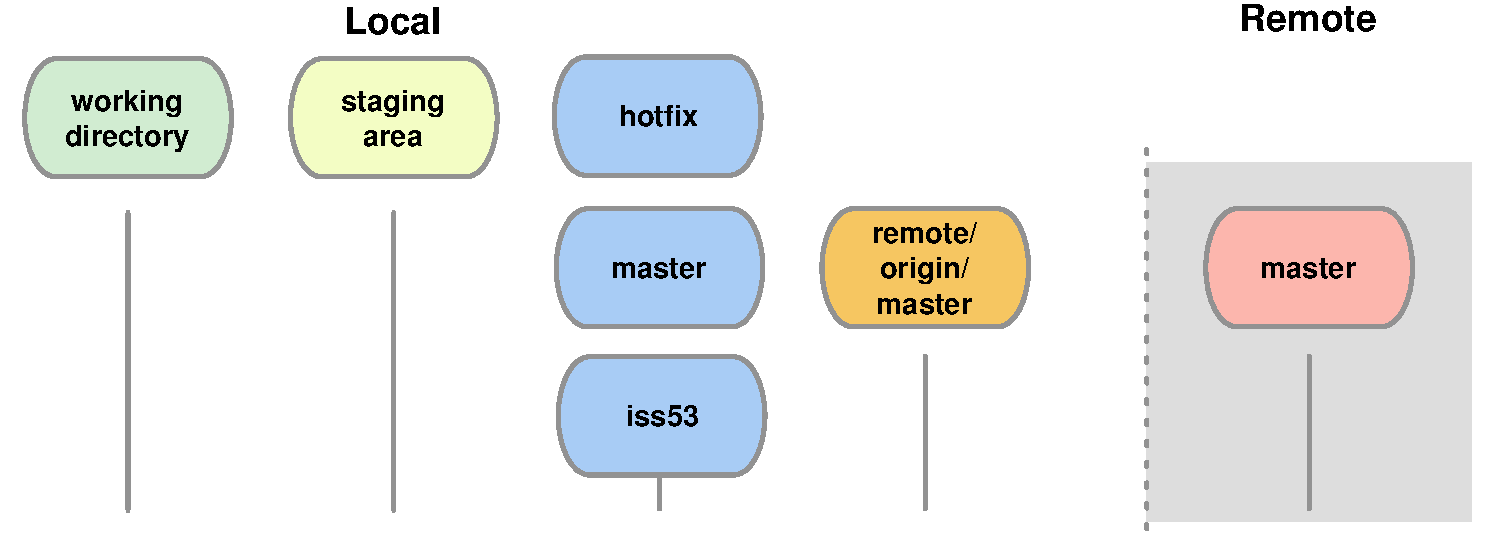
\includegraphics[width=7cm]{A2023.LavoroCondiviso/git-checkout2}
  \end{center}
\end{frame}

\begin{frame}{\centerline{Dinamica del branching -- ulteriori branch (1/3)}}
  \begin{columns}
    \begin{column}{0.6\linewidth}
      \begin{center}
        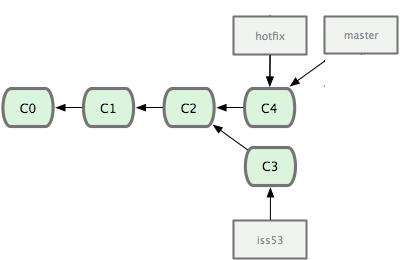
\includegraphics[width=6.5cm]{A2023.LavoroCondiviso/18333fig0314c-tn}
      \end{center}
    \end{column}
    \begin{column}{0.45\linewidth}
      \begin{center}
        \texttt{\textbf{git checkout master}}\\
        \texttt{\textbf{git merge hotfix}}\\
      \end{center}
    \end{column}
  \end{columns}
  \begin{center}
    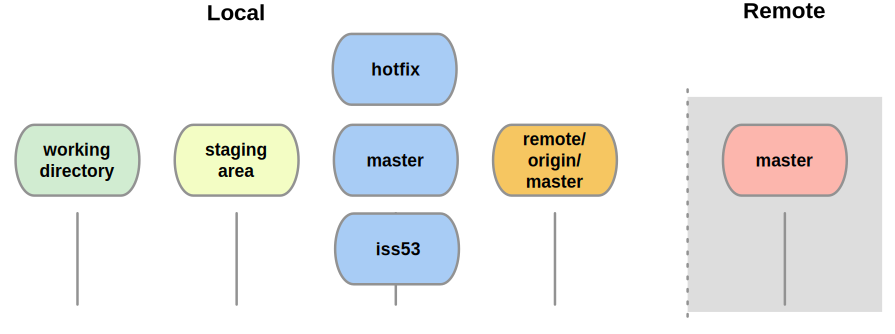
\includegraphics[width=8cm]{A2023.LavoroCondiviso/git-branch2}
  \end{center}
\end{frame}

\begin{frame}{\centerline{Dinamica del branching -- ulteriori branch (2/3)}}
  \begin{columns}
    \begin{column}{0.6\linewidth}
      \begin{center}
        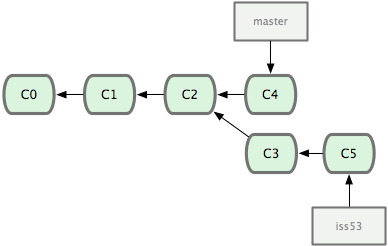
\includegraphics[width=6.5cm]{A2023.LavoroCondiviso/18333fig0315-tn}
      \end{center}
    \end{column}
    \begin{column}{0.4\linewidth}
      \begin{center}
        \texttt{\textbf{git checkout iss53}}\\
        \texttt{\textbf{git commit (C5)}}
      \end{center}
    \end{column}
  \end{columns}
  \begin{center}
    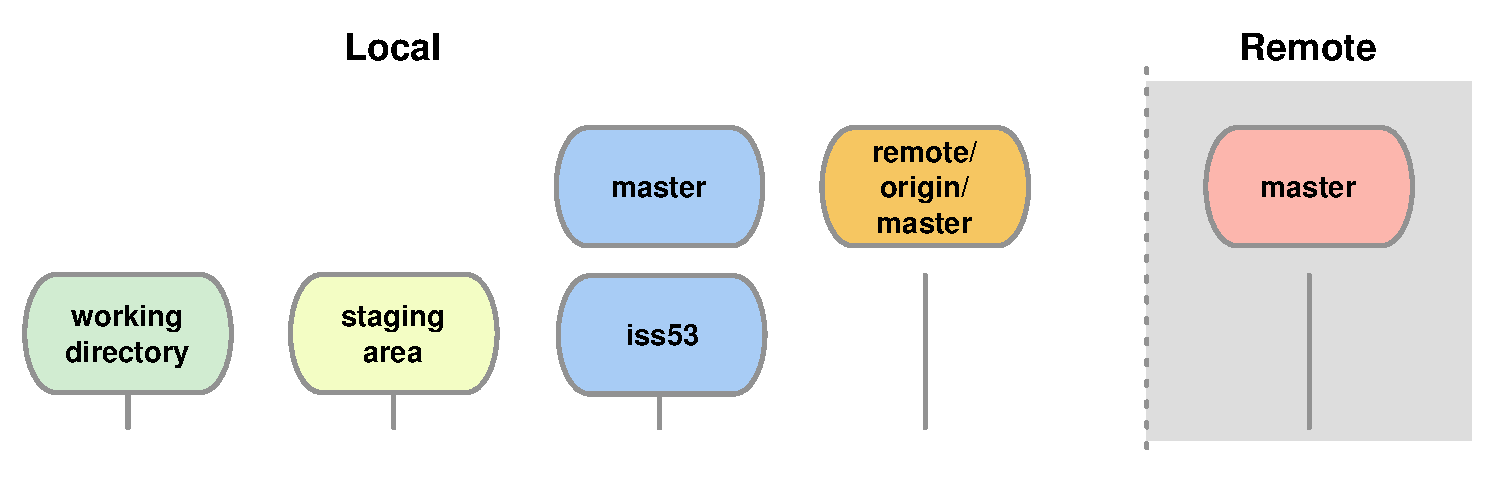
\includegraphics[width=8cm]{A2023.LavoroCondiviso/git-checkout}
  \end{center}
\end{frame}

\begin{frame}{\centerline{Dinamica del branching -- ulteriori branch (3/3)}}
  \begin{columns}
    \begin{column}{0.6\linewidth}
      \begin{center}
        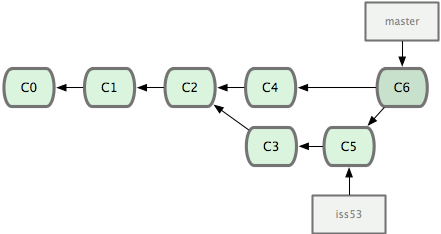
\includegraphics[width=6.5cm]{A2023.LavoroCondiviso/18333fig0317-tn}
      \end{center}
    \end{column}
    \begin{column}{0.45\linewidth}
      \begin{center}
        \texttt{\textbf{git checkout master}}\\
        \texttt{\textbf{git merge iss53}}
      \end{center}
    \end{column}
  \end{columns}
  \begin{center}
    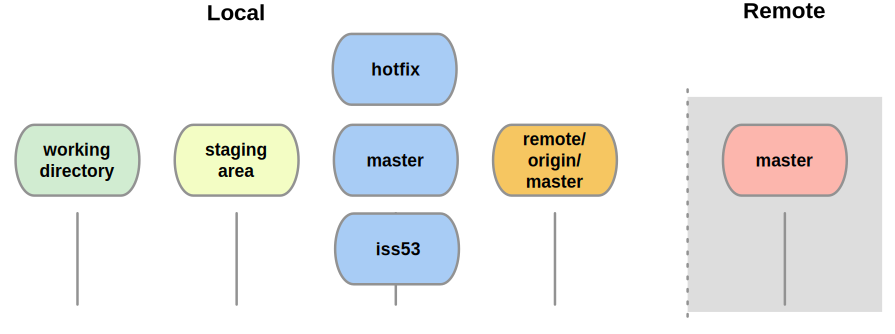
\includegraphics[width=8cm]{A2023.LavoroCondiviso/git-branch2}
  \end{center}
\end{frame}


\begin{frame}{\centerline{Contribuire a un progetto via GitHub}}
  \begin{figure}
    \centering
    Scenario 3: Contribuire a un progetto software localizzato su
    \textbf{GitHub}.
  \end{figure}
\end{frame}

\begin{frame}{\centerline{GitHub (1/2)}}
  \textbf{D:} Avete mai sentito parlare di GitHub?
  \begin{center}
      
  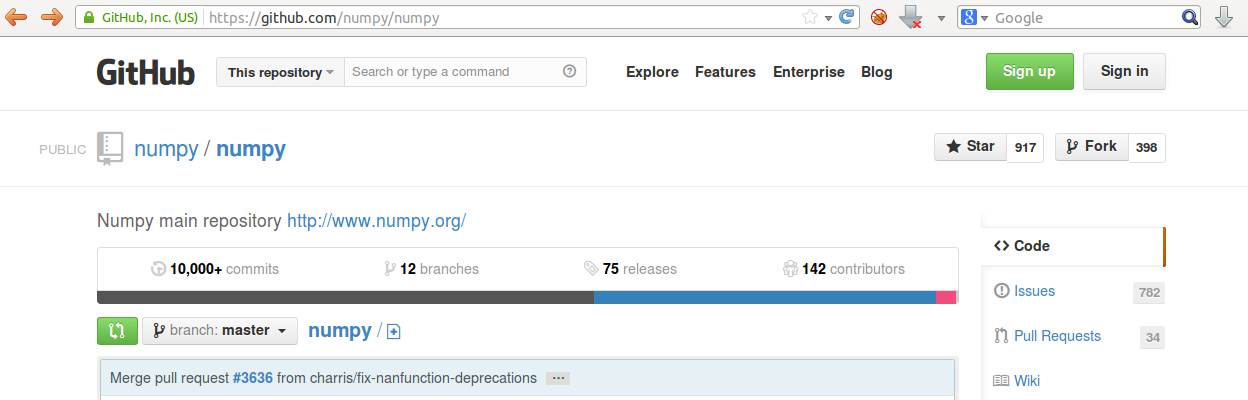
\includegraphics[width=12cm]{A2023.LavoroCondiviso/github}
    \end{center}

\end{frame}

\begin{frame}{\centerline{GitHub (2/2)}}
  \begin{block}{Che cos'\`{e} GitHub?}
    \begin{itemize}
    \item Wikipedia (tradotto): \emph{``GitHub \`{e} un servizio di hosting basato sul web che usa \git~ per progetti di sviluppo software''}.
    \item 200 milioni di repository (Giugno 2022).
    \item Commerciale...
    \item ... ma non ostile ai progetti Free, Libre, and Open Source.
    \item Per software si intendono non solo i programmi, ma qualunque entit\`{a} rappresentabile in forma digitale ...
    \item ... per\`{o} Per quello memorizzabili in ``formato testo'' il sistema \textit{funziona meglio}
    \item per scrivere un libro con LaTeX funziona benissimo
    \end{itemize}
  \end{block}
\end{frame}


\begin{frame}{\centerline{Contribuire a progetti tramite GitHub}}
  \begin{block}{Assunti}
    \begin{itemize}
    \item Usi o conosci un software e ti senti pronto a contribuirvi
    \item Il progetto software viene ospitato all'url \url{http://github.com}
    \end{itemize}
  \end{block}
  \begin{block}{Idea intuitiva}
    \begin{itemize}
    \item Non si fanno \textbf{ push} dei cambiamenti nel repository principale
    \item Invece si crea una copia pubblica del repository principale you create a public copy (\textbf{fork}) ...
    \item ... e poi si fa push dei cambiamenti in quella.
    \item Infine si chiede ai proprietari del progetto (del repository principale) se a loro piacciono tali cambiamenti e se vogliono fare un merge di essi (\textbf{pull request}).
    \end{itemize}
  \end{block}
\end{frame}

\begin{frame}{\centerline{Non \`{e} per tutti!}}
\begin{center}
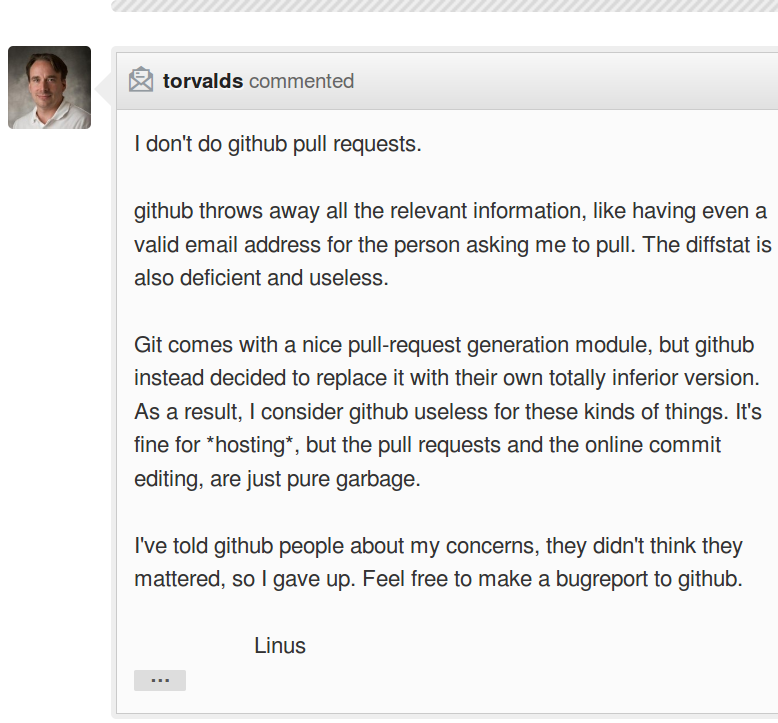
\includegraphics[width=7cm]{A2023.LavoroCondiviso/linus-on-pull-requests}
  \url{https://github.com/torvalds/linux/pull/17}
\end{center}
\end{frame}

\begin{frame}{\centerline{Ricetta (1/4)}}
  \begin{enumerate}
  \item \textbf{Registrarsi} su \url{http://github.com}
  \item \textbf{Visitare} la pagina GitHub del progetto software e fare un \textbf{Fork} di esso:
  \end{enumerate}
\begin{center}
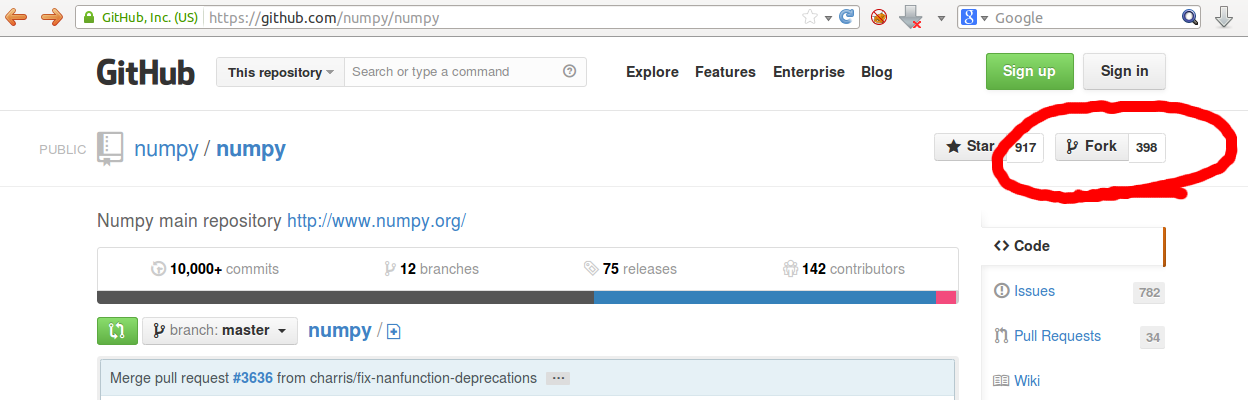
\includegraphics[width=12cm]{A2023.LavoroCondiviso/github-fork}
\end{center}

\end{frame}

\begin{frame}{\centerline{Ricetta (2/4)}}
  \begin{enumerate}
  \setcounter{enumi}{2}
  \item Fare un \textbf{clone} della propria copia del progetto sul proprio computer
    \begin{center}
        \texttt{\textbf{git clone git@github.com:<login>/<project>.git}}
    \end{center}
  \item Creare un \textbf{branch} per ospitare i propri miglioramenti.
    \begin{itemize}
    \item \texttt{\textbf{git branch <new-feature>}} 
\includegraphics[height=0.55cm]{A2023.LavoroCondiviso/github-branch}
    \item \texttt{\textbf{git checkout <new-feature>}}
    \end{itemize}
  \end{enumerate}
\end{frame}

\begin{frame}{\centerline{Ricetta (3/4)}}
  \begin{enumerate}
    \setcounter{enumi}{4}
  \item Aggiungere i propri miglioramenti.
    \begin{itemize}
    \item \texttt{\textbf{git add <new-file>}}
    \item \texttt{\textbf{git commit -m ...}}
    \end{itemize}    
  \item Fare un \textbf{push} dei propri miglioramenti.
    \begin{center}
      \texttt{\textbf{git push origin <new-feature>}}
    \end{center}
  \end{enumerate}
\end{frame}

\begin{frame}{\centerline{Ricetta (4/4)}}
  \begin{enumerate}
    \setcounter{enumi}{6}
  \item Mandare una richiesta di \textbf{pull}.
    
\includegraphics[height=0.55cm]{A2023.LavoroCondiviso/github-compare-and-pull-request}
    \begin{center}
      \hbox{\hspace{-0cm}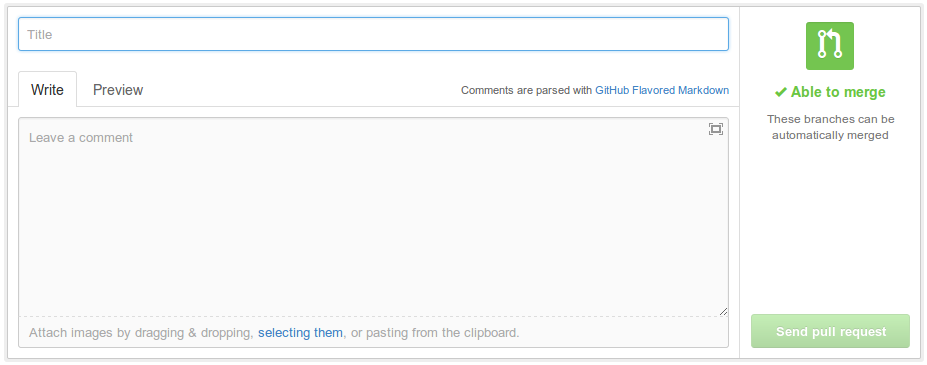
\includegraphics[width=12cm]{A2023.LavoroCondiviso/github-pull-request}}
    \end{center}
  \end{enumerate}
\end{frame}


\begin{frame}{\centerline{Spiegazione dettagliata}}
  \includegraphics<1>[width=11cm]{A2023.LavoroCondiviso/pull-request-0}
  \includegraphics<2>[width=11cm]{A2023.LavoroCondiviso/pull-request3-1}
  \includegraphics<3>[width=11cm]{A2023.LavoroCondiviso/pull-request3-2}
  \includegraphics<4>[width=11cm]{A2023.LavoroCondiviso/pull-request3-3}
  \includegraphics<5>[width=11cm]{A2023.LavoroCondiviso/pull-request3-4}
  \includegraphics<6>[width=11cm]{A2023.LavoroCondiviso/pull-request3-5}
  \includegraphics<7>[width=11cm]{A2023.LavoroCondiviso/pull-request-4}
  \includegraphics<8>[width=11cm]{A2023.LavoroCondiviso/pull-request-5}
  \begin{center}
    \only<1>{C'\`{e} un progetto ospitato su un repository GitHub remoto (\textbf{upstream}). Si vuole contribuire a migliorarlo.}
    \only<2>{Quindi si fa un \textbf{fork} per crearne una copia (remota):\\
        \textcolor{grey}{\texttt{\textbf{git clone -{}-bare
            <UPSTREAM\_URL>}}}}
    \only<3>{Ora si clona la copia sul computer locale:\\
      \texttt{\textbf{git clone <ORIGIN\_URL>}}}
    \only<4>{\texttt{\textbf{git remote add upstream
          <UPSTREAM\_URL>}}\\
    \texttt{\textbf{git fetch upstream}}}
    \only<5>{\texttt{\textbf{git branch new-feature upstream/master}}\\
      \texttt{\textbf{git checkout new-feature}}}
    \only<6>{\texttt{\textbf{git add ... \\git commit ...}}}
    \only<7>{Pubblica le nuove caratteristiche (feature):\\
      \texttt{\textbf{git push origin new-feature}}} 
    \only<8>{Notifica i proprietari del repository principale sulle nuove caratteristiche 
      (\texttt{\textbf{new-feature}})\\
      loro potranno fare: \texttt{\textbf{git fetch}} + (eventualmente)
      \texttt{\textbf{git merge}}}
  \end{center}
\end{frame}

% \begin{frame}{Contributing through GitHub. Demo.}
%   \begin{center}
%     Demo: Live.
%   \end{center}
% \end{frame}

% \begin{frame}{Extras. \alert{OPTIONAL}}
%   \begin{itemize}
%   \item Local branching + demo.
%   \item Setting up a remote shared repository + demo.
%   \end{itemize}
% \end{frame}

\begin{frame}{\centerline{Creare un repository remoto/condiviso (1/4)}}
  \begin{center}
    \textcolor{orange}{SCOPO: voglio condividere il mio repository locale in modo che altri possano fare \texttt{\textbf{push}}.}
  \end{center}
  ``Perch\'{e} non posso semplicemente cambiare i permessi nel mio repository \textbf{locale}?''
  \begin{itemize}
  \item Certamente si pu\`{o}...
  \item ...ma i tuoi colleghi non potranno fare push (\alert{read-only}).
  \end{itemize}
  \begin{center}
    Per poterlo avere con permessi \alert{read-write}: occorre fare un repository \textbf{remoto}
    \emph{condiviso}.
  \end{center}
\end{frame}


\begin{frame}{\centerline{Creare un repository remoto/condiviso (2/4)}}
  \begin{center}
    \textcolor{orange}{SCOPO: voglio condividere il mio repository locale in modo che altri possano fare \texttt{\textbf{push}}.}
  \end{center}

  \begin{figure}
    \centering
    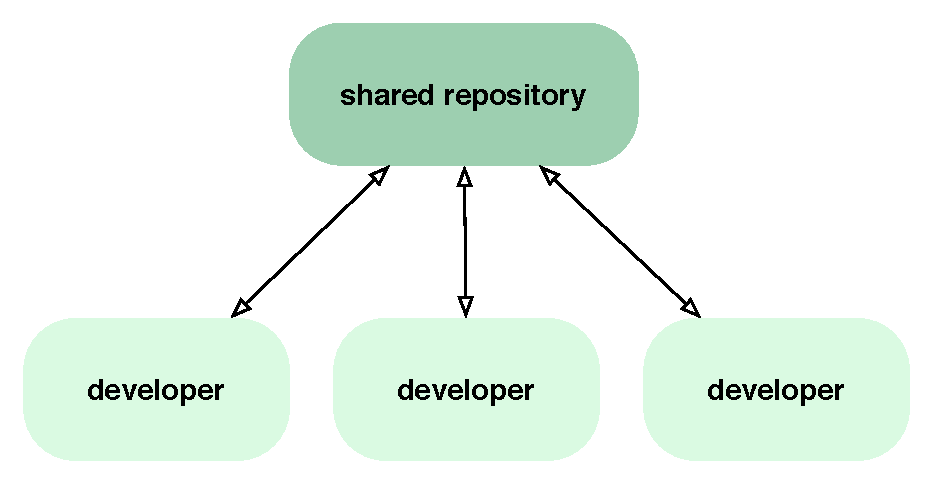
\includegraphics[width=8cm]{A2023.LavoroCondiviso/workflow-a}
  \end{figure}
\end{frame}


\begin{frame}{\centerline{Creare un repository remoto/condiviso (3/4)}}
  \begin{center}
    \textcolor{orange}{SCOPO: voglio condividere il mio repository locale in modo che altri possano fare \texttt{\textbf{push}}.}
  \end{center}

  Hai un repository locale e lo vuoi condividere da 
  (\texttt{\textbf{ssh}}) da un server remoto su cui i tuoi colleghi hanno gi\`{a} accesso
  \begin{block}{Sul server \emph{remoto} crea un repository 
      \textbf{vuoto}+\textbf{condiviso}:}
    \begin{itemize}
    \item \texttt{\textbf{mkdir newproject}}
    \item genera i permessi necessari per il \emph{gruppo}: \texttt{\textbf{chmod g+rws newproject}}
    \item \texttt{\textbf{cd newproject}}
    \item \texttt{\textbf{git \alert{-{}-bare} init \alert{-{}-shared=group}}}
    \end{itemize}
  \end{block}

\end{frame}

\begin{frame}{\centerline{Creare un repository remoto/condiviso (4/4)}}
  \begin{center}
    \textcolor{orange}{SCOPO: voglio condividere il mio repository locale in modo che altri possano fare \texttt{\textbf{push}}.}
  \end{center}

  \begin{block}{Sulla macchina \emph{locale} fai push del tuo repository verso quello remoto:}
    \begin{itemize}
    \item \texttt{\textbf{git remote add origin }}
          \begin{center}
            \texttt{\textbf{ssh://remote.com/path/newproject}}
      \end{center}
    \item \texttt{\textbf{git push \alert{-u} origin master}}
    \end{itemize}
  \end{block}
  E poi alla fine ognuno pu\`{o} fare un clone del repository condiviso:
  \begin{center}
    \texttt{\textbf{git clone ssh://remote.com/path/newproject}}
  \end{center}
\end{frame}


\begin{frame}{\centerline{Crediti}}
  \begin{itemize}
  \item \textbf{Rike-Benjamin Schuppner}
  \item Zbigniew J\k{e}drzejewski-Szmek
  \item Tiziano Zito
  \item Bastian Venthur
  \item \url{http://progit.com}
  \item \url{apcmag.com}
  \item \url{lwn.net}
  \item \url{http://www.markus-gattol.name/ws/scm.html}
  \item \url{http://matthew-brett.github.io/pydagogue/gitwash/git_development.html}
  \end{itemize}
\end{frame}

\begin{frame}{\centerline{Se si vuole sapere di pi\`{u} su \git}}
  Sul funzionamento di \git :
  \begin{itemize}
  \item \git foundations, di Matthew Brett:
    \small
    \url{http://matthew-brett.github.com/pydagogue/foundation.html}
  \item  The \git parable, by Tom Preston-Werner:
    \small
  \url{http://tom.preston-werner.com/2009/05/19/the-git-parable.html}
  \end{itemize}
  Ottime guide:
  \begin{itemize}
  \item ``Pro Git'' book: \url{http://git-scm.com/book} (gratis)
  \item \git magic: \url{http://www-cs-students.stanford.edu/~blynn/gitmagic/}
  \end{itemize}
  Per contribuire a un progetto ospitato su  GitHub:
  \begin{itemize}
  \item ``Gitwash'', di Matthew Brett:
    \small
    \url{http://matthew-brett.github.io/pydagogue/gitwash/git_development.html}
  \end{itemize}
\end{frame}

\begin{frame}{\centerline{Materiale interessante}}
Gource:
  \begin{center}
    \url{http://code.google.com/p/gource/}
  \end{center}
\end{frame}


\begin{frame}{\centerline{Licenza per la parte su Git}}
  \begin{center}
    Copyright Emanuele Olivetti, 2014
  \end{center}
  \vspace{1em}
  \begin{center}
    Questa distribuzione viene distribuita con la licenza\\
    \textbf{Creative Commons \emph{Attribution} 3.0}\\
    \url{https://creativecommons.org/licenses/by/3.0/}
  \end{center}
  \vspace{1em}
  \begin{center}\small
    I diagrammi per il branching sono presi da \emph{Pro
      Git}, (copyright S.Chacon, 2009) e sono distribuuiti con la licenza Creative Commons 3.0 Attribution-Non Commercial-Share Alike.
  \end{center}
\end{frame}


\begin{frame}
{\centerline{Domande?}}
\vspace{1cm}
\begin{center}
    \LARGE{Fine della seconda lezione.}
\end{center}

\end{frame}

\end{document}


